\chapter{FLC100 shield assembly}

\section{Introduction}
The FLC100 shield is an Arduino ``shield'' which interfaces the
microcontroller to the FLC100 fluxgate magnetometer sensor, if
necessary translating logic levels. It is also responsible for
generating the correct operating voltage for the
microcontroller. There is more than one version of this board, be sure
to use the instructions appropriate to your version.

\section{FLC100 shield version 1.0}

\subsection{Description}

The FLC100 shield version 1.0 operates at \volt{3.3}. \textbf{Do not
  attempt to use it with standard Arduino boards which are operated at
  \volt{5}.} The shield houses the XRF radio module, the boost power
supply (which creates the \volt{3.3} supply for the microcontroller
and radio) and the \volt{3.3} -- \volt{5} level shifters.

There are both through-hole and surface mount versions of the boost
power supply. It is suspected that the through-hole version causes
\rfi\ since the radio module often fails to receive messages. This
problem was not apparent on the prototype board. The surface-mount
version has no such problems and is the option which should be
used. It is also cheaper and more efficient.

There is an option to fit a FLC100 sensor directly to the circuit
board. This option is not used because the FLC100 is slightly
temperature sensitive and better performance is obtained by
positioning the sensor below ground. Whilst the board provides an
option to fit an MCP3424 \adc\ and MAX619 charge-pump power supply they
are also fitted remotely, below ground, for reasons of temperature
stability.


\begin{figure}
  \centering
  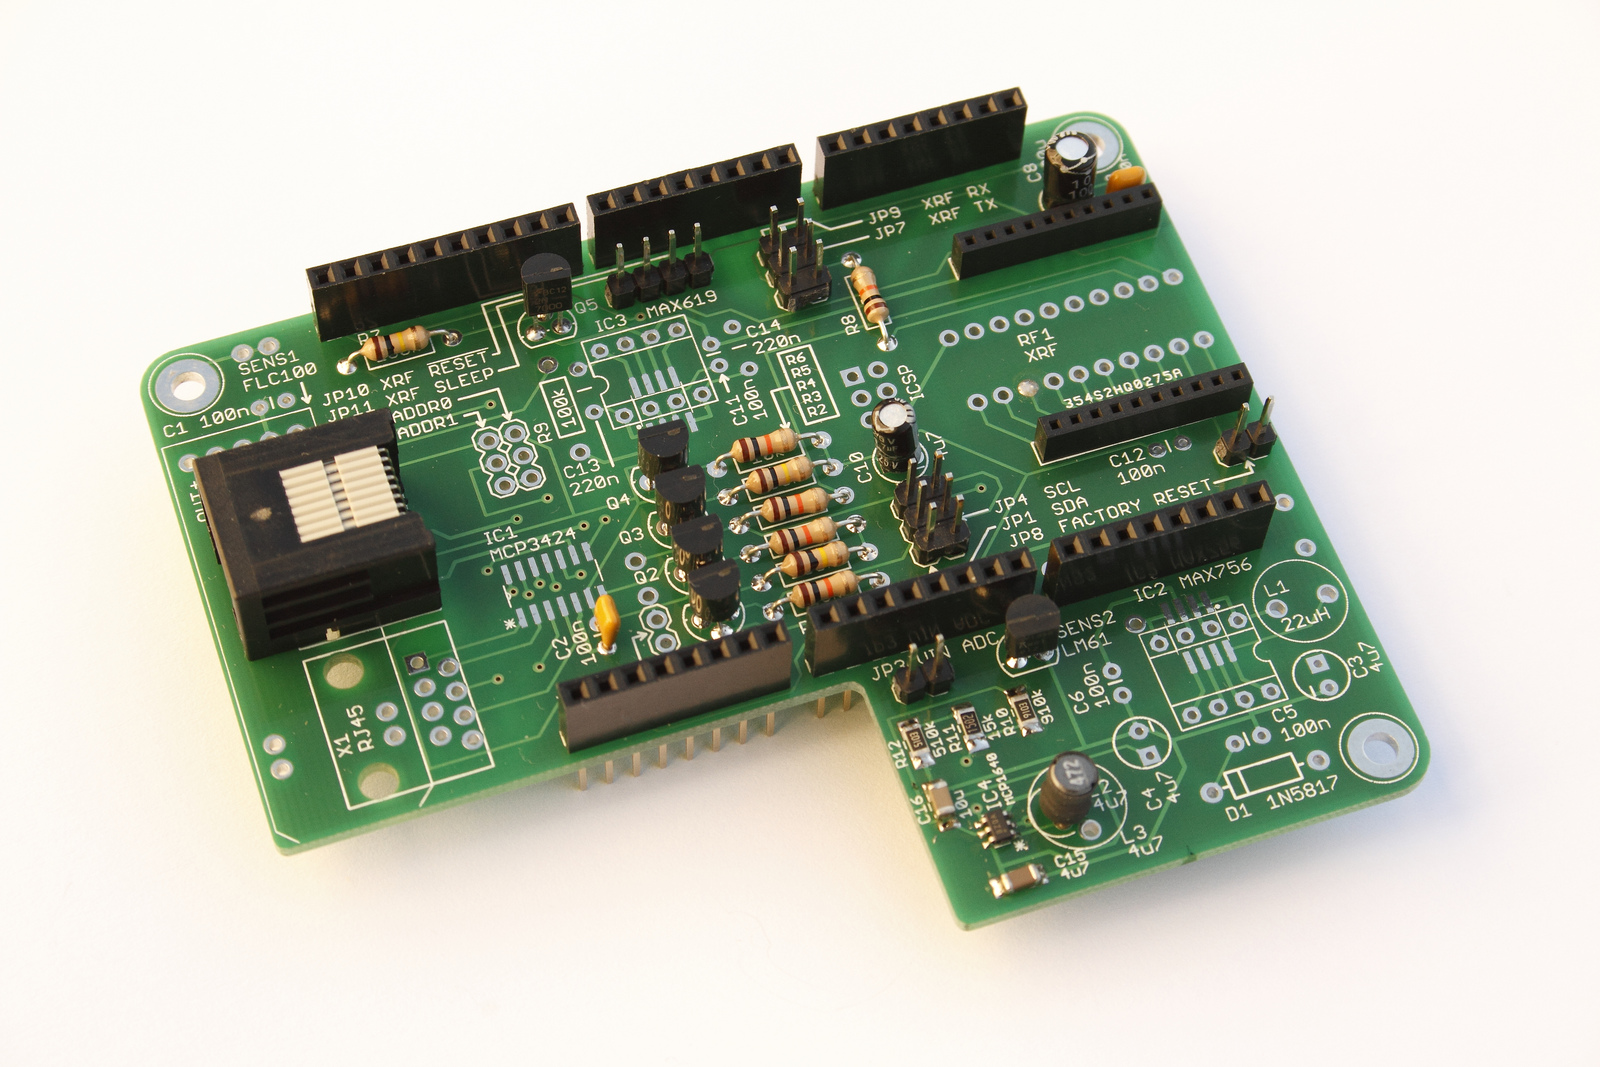
\includegraphics[keepaspectratio,width=\textwidth]{%
    images/flc100-shield}
  \caption[Completed FLC100 shield]{Completed FLC100 shield, except
    for fitting shunts onto the jumpers. %
    \photoCredit{Steve Marple}{\ccBySaTwo}{%
      http://www.flickr.com/photos/stevemarple/10787109594/}}
  \label{fig:flc100-v1.0}
\end{figure}

\subsection{Order of assembly}
\begin{buildorder}
\item IC4 (MCP1640).
\item R12 (\kohm{510}).
\item R11 (\kohm{15}).
\item R10 (\kohm{910}).
\item C15 (\uF{4.7}).
\item C16 (\uF{10}).
\item \SI{2}{\milli\metre} 10~way connectors for RF1. Ensure they are
  fitted flush to the \pcb.
\item R1, R3, R4, R6, R8 (\kohm{10}).
\item R2, R5, R7 (\kohm{100}).
\item C2, C7, C9 (\nF{100}).
\item C10 (\uF{4.7}).
\item C8 (\uF{100}).
\item L2 (\uH{4.7}). The shorter lead should be connected to pin~1,
  which is the hole nearest the edge of the \pcb. Although the
  orientation of inductors is normally ignored communication with the
  manufacturer revealed that the shorter lead indicates the start of
  the winding. This arrangement is preferred to help minimise \rfi.
\item Stacking connectors, five 8~way and one 10~way. Ensure they are
  fitted flush to the \pcb; solder one end first, then the other
  end. Only when you are happy they are flush should you solder the
  remaining pins.
\item JP1, JP4 ($2 \times 3$ jumper).
\item JP7, JP9 ($2 \times 3$ jumper).
\item JP10, JP11 ($1 \times 4$ jumper).
\item JP3 ($1 \times 2$ jumper).
\item JP8 ($1 \times 2$ jumper).
\item X2 (RJ45 connector).
\item Modify the \pcb\ by adding a link wire from the XRF ONSLEEP
  status pin to D23. See figure~\ref{fig:flc100-sleep-status-mod}.
\item Q1, Q2, Q3, Q4, Q5 (2N7000).
\end{buildorder}

\begin{figure}
  \centering
  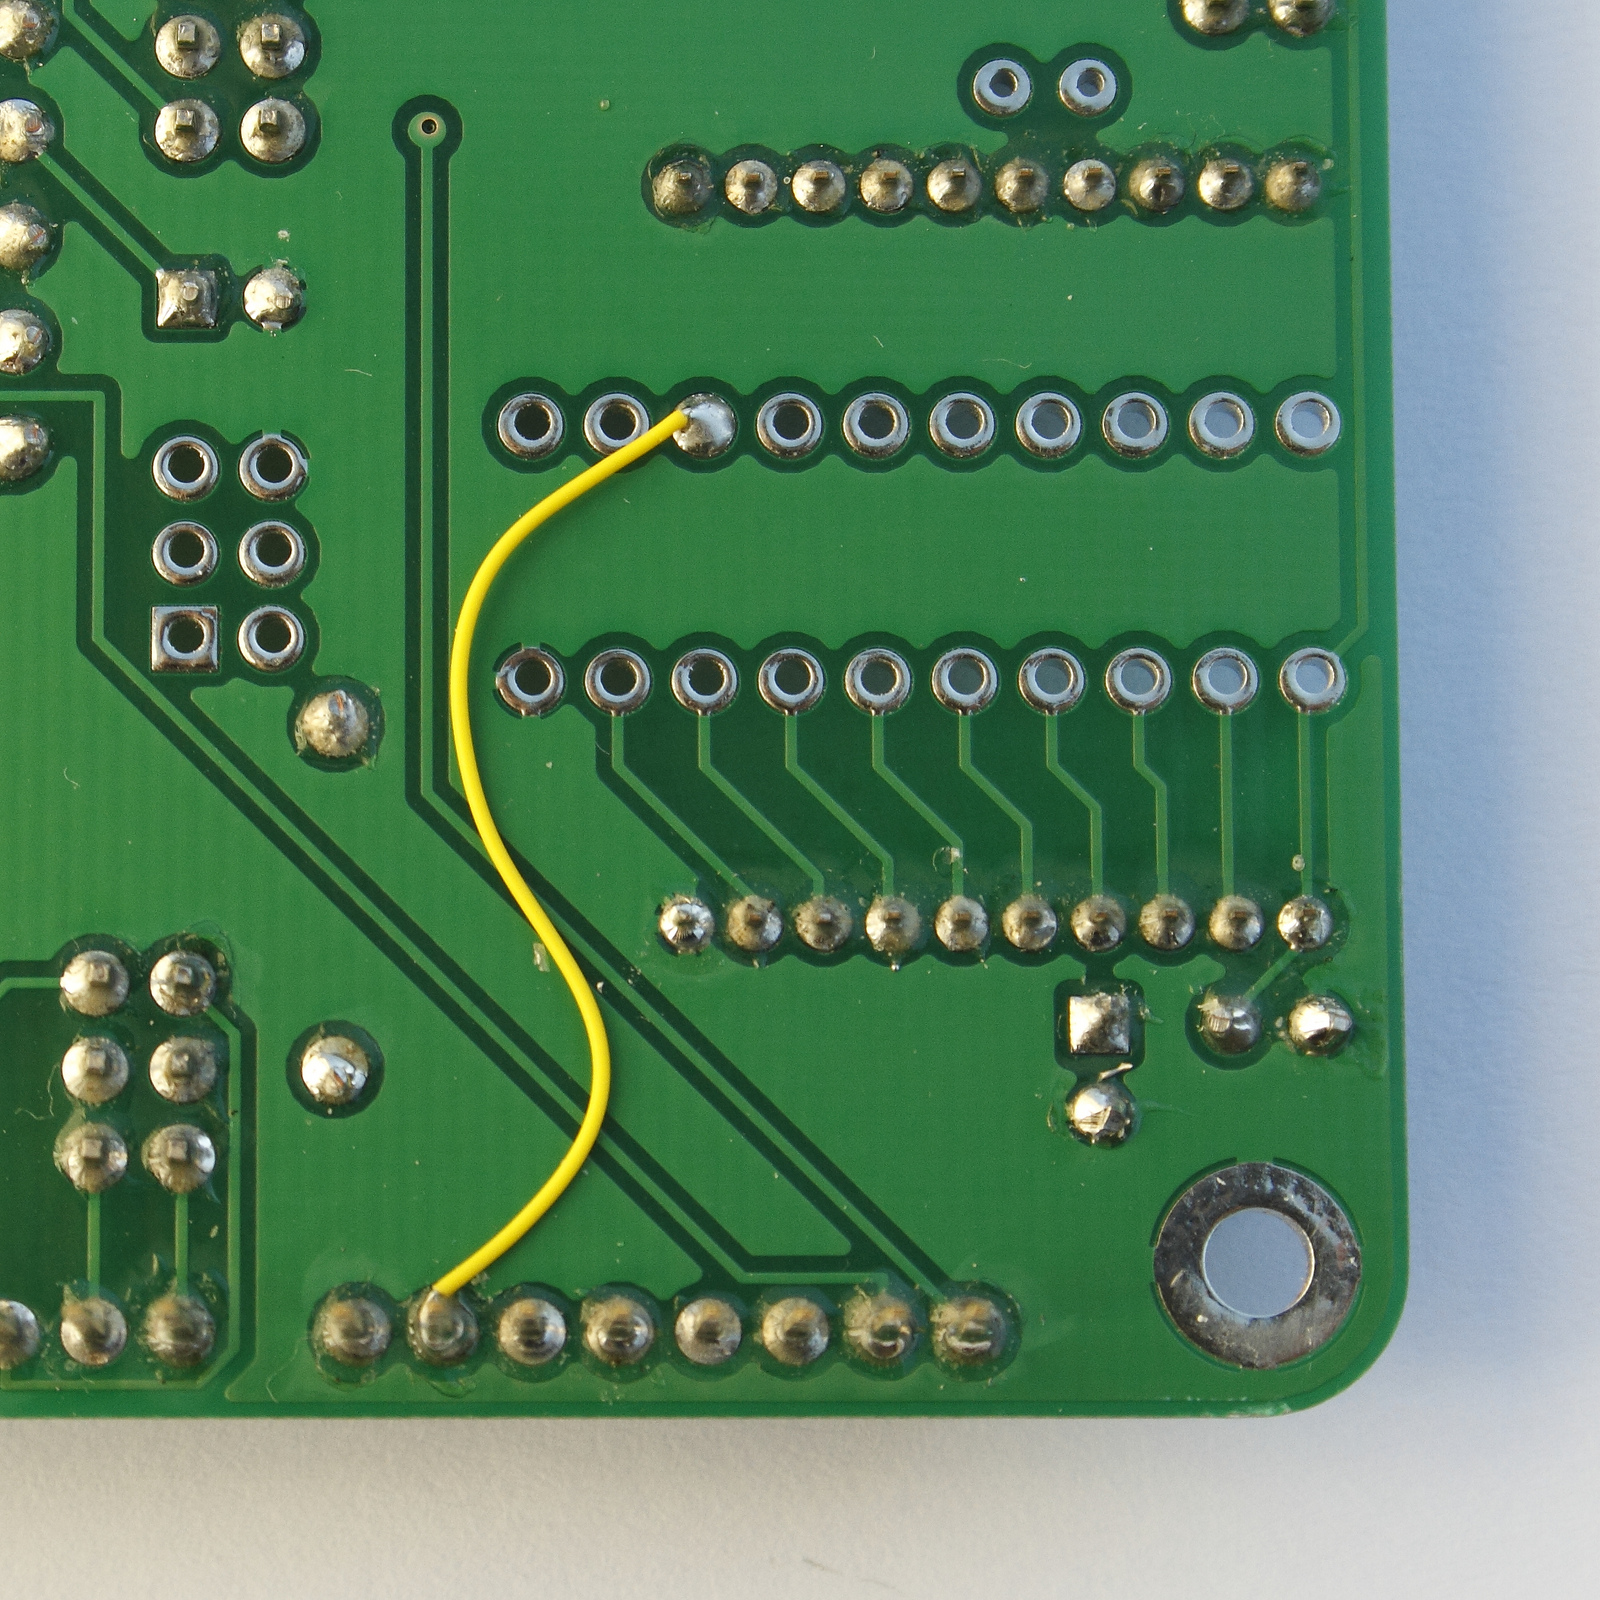
\includegraphics[keepaspectratio,width=10cm]{%
    images/flc100-sleep-status-mod}
  \caption[Modification to monitor sleep status of the XRF radio module]{%
    Modification to monitor sleep status of the XRF radio module.
    \photoCredit{Steve Marple}{\ccBySaTwo}{%
      http://www.flickr.com/photos/stevemarple/10786910376/}}
  \label{fig:flc100-sleep-status-mod}
\end{figure}


Fit shunts to JP10, JP11, JP3. Fit shunts to JP7 and JP9, to the two
connectors furthest from the edge of the \pcb. \textbf{Do not fit the
  shunts so that they bridge between JP7 and JP9}.

If the microcontroller board has dedicated \itwoc\ connections (\eg
Calunium v2.0 or later), then no shunts should be fitted to JP1 and
JP4. If the microcontroller has \itwoc\ connections in the standard
Arduino Mega positions (\eg, Calunium v1.0, Arduino Mega, Arduino Mega
2560) then fit shunts to JP1 and JP4 to the two connectors closest to
C10, otherwise fit shunts to JP1 and JP4 to the two connectors closest
to the stacking connectors. \textbf{In no circumstances should the
  shunts bridge between JP1 and JP4}.

Leave JP8 open circuit. It is fitted only when the XRF1 radio module
must be forced to use the default factory configuration.

\begin{landscape}
  \begin{figure}[p]
    \centering
    \includegraphics[keepaspectratio,width=28cm,height=16cm]{%
      calunium-mag/images/FLC100-shield-v1-0-sch}
    \caption{FLC100 shield v.~1.0 circuit diagram.}
    \label{fig:flc100-shield-v1.0-cct-diag}
  \end{figure}
\end{landscape}

\section{FLC100 shield version 2.0}

\subsection{Description}

The FLC100 shield version 2.0 can operate at either \volt{3.3} or
\volt{5}. This enables the board to be used either for battery-powered
systems, with the microcontroller and radio operating at \volt{3.3} or
with the standard Arduino Ethernet shield which requires the shield
and microcontroller to operate at \volt{5}. When used in conjunction
with the Arduino Ethernet shield it is assumed that the \PoE\ module
is fitted. The operating voltage chosen during construction determines
which components are fitted.

The shield can also be used for cloud detection, for which it supports
the operation of an MLX90614 non-contact \ir\ thermometer, HIH61xx
humidity and ambient temperature sensor, and Embedded Adventures
lightning sensor module. These functions are outside of the scope of
this document and will not be described here.

\subsubsection{Battery operation}
When built for battery operation the shield houses the XRF radio
module, the boost power supply (which creates the \volt{3.3} supply
for the microcontroller and radio) and the \volt{3.3} -- \volt{5}
level shifters. The boost regulator can be built onto the \pcb\ using
discrete components. A simpler alternative which avoids the need to
solder small surface mount components is to fit a ready-built
third-party module.


\subsubsection{Power over Ethernet operation}
If used in conjunction with the Ethernet shield the
XRF radio module and boost power supply are not fitted. The Ethernet
shield provides a \volt{9} output onto the \texttt{Vin} pin,
requiring that a linear or buck regulator is fitted for \volt{5} operation.

\subsection{Order of assembly}
\subsubsection{Battery-powered version}

\warningbox{Build instructions for the battery-powered option of the
  FLC100 shield version 2.0 are untested. Proceed with caution.}

Order of assembly for the battery-powered version.

If using the on-board surface-mount boost regulator fit:
\begin{buildorder}
\item IC4 (MCP1640).
\item R19 (\kohm{510}).
\item R18 (\kohm{15}).
\item R17 (\kohm{910}).
\item C4 (\uF{4.7}).
\item C5 (\uF{10}).
\end{buildorder}

For all battery-powered versions fit:

\begin{buildorder*}
\item \SI{2}{\milli\metre} 10~way connectors for RF1. Ensure they are
  fitted flush to the \pcb.
\item R4 (\kohm{1}).
\item R1, R3, R5, R7, (\kohm{10}).
\item R2, R6 (\kohm{100}).
\item R8 (\Mohm{1}).
\item C1, C3 (\nF{100}).
\item C2, C9 (\uF{100}).
\item C6 (\uF{100} \volt{25}).
\item L1 (\uH{4.7}). The shorter lead should be connected to pin~1,
  which is the hole nearest the edge of the \pcb. Although the
  orientation of inductors is normally ignored communication with the
  manufacturer revealed that the shorter lead indicates the start of
  the winding. This arrangement is preferred to help minimise \rfi.
\item Stacking connectors, five 8~way and one 10~way. Ensure they are
  fitted flush to the \pcb; solder one end first, then the other
  end. Only when you are happy they are flush should you solder the
  remaining pins.
\item JP2 ($1 \times 2$ jumper).
\item JP3, JP5 ($1 \times 3$ jumper).
\item JP4, ISP header ($2 \times 3$ jumper).
\item X1 (RJ45 connector).
\item Q1, Q2, Q3, Q4, Q5 (2N7000). Fit last to minimise risk of damage
  from \esd.
\end{buildorder*}

If using an external boost regulator fit:
\begin{buildorder*}
\item Boost regulator module (Ciseco PowerPOD NCP1402 3V3).
\end{buildorder*}


\subsubsection[Order of assembly: PoE version]{%
  Order of assembly: \protect\PoE\ version}

\warningbox{Build instructions for \PoE\ option of the FLC100 shield
  version 2.0 are untested. Proceed with caution.}  Order of assembly
for the \PoE\ version.
\begin{buildorder}
\item R1, R3, R5, R7, (\kohm{10}).
\item R2, R6 (\kohm{100}).
\item C1, C3 (\nF{100}).
\item C7 (\uF{4.7}).
\item C2, C9 (\uF{100}).
\item C6 (\uF{100} \volt{25}).
\item L1 (\uH{4.7}). The shorter lead should be connected to pin~1,
  which is the hole nearest the edge of the \pcb. Although the
  orientation of inductors is normally ignored communication with the
  manufacturer revealed that the shorter lead indicates the start of
  the winding. This arrangement is preferred to help minimise \rfi.
\item Stacking connectors, five 8~way and one 10~way. Ensure they are
  fitted flush to the \pcb; solder one end first, then the other
  end. Only when you are happy they are flush should you solder the
  remaining pins.
\item JP3 ($1 \times 3$ jumper).
\item JP4, ISP header ($2 \times 3$ jumper).
\end{buildorder}

If the master \pcb\ of the FLC100 remote sensor is version 2.0 and it
will be fitted with a linear regulator (MCP1702) then JP5 can be
omitted. Otherwise fit:
\begin{buildorder*}
\item JP5 ($1 \times 3$ jumper).
\item Add shunt to JP5, connect the centre pin to \texttt{Vin} if a
  linear regulator is fitted to the master FLC100 remote sensor \pcb;
  connect to \texttt{+3V3} if the MAX619 boost regulator is used on
  the master FLC100 remote sensor \pcb.
\end{buildorder*}


The connector to the remote sensor \pcb{}(s) can be either RJ11 or
RJ45. The RJ45 has the advantage that a standard (straight-through)
Ethernet cable can be used. However it has the disadvantage that it is
possible to inadvertently fit the \PoE\ Ethernet connection into the
wrong socket.
\begin{buildorder*}
\item X1 (RJ45 connector) or X2 (RJ11 connector). 
\end{buildorder*}

Add shunts to jumper blocks\marginpar{to complete}.
\begin{buildorder*}
\item Fit 3 shunts to JP4, in the positions marked on the silkscreen.
\item Fit a shunt to JP5, linking the centre pin with \texttt{+5V}.
\end{buildorder*}

\warningbox{If JP2 is fitted \textbf{do not} fit a shunt when used for
  \PoE\ operation, it will damage the microcontroller. Measurement of
  the input voltage can only be performed when $\textrm{V}_{\textrm{in}} \le
  \textrm{V}_{\textrm{cc}}$.}

Finally fit last to minimise risk of damage from \esd.
\begin{buildorder*}
\item Q1, Q2, Q3, Q4 (2N7000).
\end{buildorder*}


\subsubsection{Other variations}
If is possible (though not desirable) for the \volt{5} supply for the
remote sensor \pcb{}(s) to be generated by the FLC100 shield. To enable
this fit JP1 and add a shunt to link the \volt{5} rails between the
\pcb{}s.


\begin{landscape}
  \begin{figure}[p]
    \centering
    \includegraphics[keepaspectratio,width=28cm,height=16cm]{%
      calunium-mag/images/FLC100-shield-v2-0-sch}
    \caption{FLC100 shield v.~2.0 circuit diagram.}
    \label{fig:flc100-shield-v2.0-cct-diag}
  \end{figure}
\end{landscape}
